\documentclass[tikz,border=2pt]{standalone}
\usepackage{amsmath,amssymb}
\usepackage{tikz}
\usetikzlibrary{arrows.meta}

\begin{document}
% A path from A to F: a sequence of distinct edges, consecutive ones sharing a vertex;
% here A-C, C-B, B-D, D-E, E-F of total length 13.
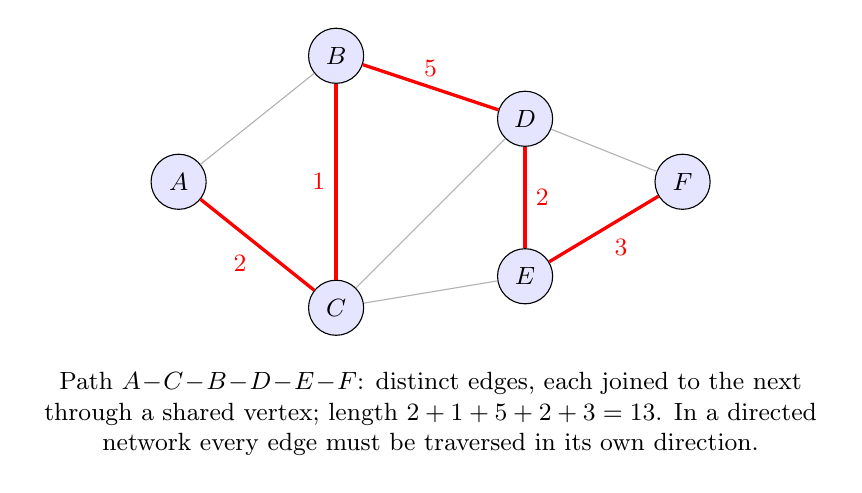
\begin{tikzpicture}[every node/.style={font=\small}, v/.style={draw, circle, fill=blue!10, minimum size=7mm, inner sep=0pt}]
	\node[v] (A) at (0,0) {$A$};
	\node[v] (B) at (2,1.6) {$B$};
	\node[v] (C) at (2,-1.6) {$C$};
	\node[v] (D) at (4.4,0.8) {$D$};
	\node[v] (E) at (4.4,-1.2) {$E$};
	\node[v] (F) at (6.4,0) {$F$};
	\foreach \a/\b in {A/B, B/D, C/D, C/E, D/F} {\draw[gray!60] (\a) -- (\b);}
	\draw[red, very thick] (A) -- (C) node[midway, below left] {$2$};
	\draw[red, very thick] (C) -- (B) node[midway, left] {$1$};
	\draw[red, very thick] (B) -- (D) node[midway, above] {$5$};
	\draw[red, very thick] (D) -- (E) node[midway, right] {$2$};
	\draw[red, very thick] (E) -- (F) node[midway, below right] {$3$};
	\node[anchor=north, align=flush center, text width=10cm] at (3.2,-2.3) {Path $A\!-\!C\!-\!B\!-\!D\!-\!E\!-\!F$: distinct edges, each joined to the next through a shared vertex; length $2+1+5+2+3=13$. In a directed network every edge must be traversed in its own direction.};
\end{tikzpicture}
\end{document}
